%%%%%%%%%%%%%%%%%%%%%%%%%%%%%%%%%%%%%%%%%%%%%%%%%%%%%%%%%%%%
%%% ELIFE ARTICLE TEMPLATE
%%%%%%%%%%%%%%%%%%%%%%%%%%%%%%%%%%%%%%%%%%%%%%%%%%%%%%%%%%%%
%%% PREAMBLE 
\documentclass[9pt,lineno,onehalfspacing]{elife}
% Use the onehalfspacing option for 1.5 line spacing
% Use the doublespacing option for 2.0 line spacing
% Please note that these options may affect formatting.
% Additionally, the use of the \newcommand function should be limited.

\usepackage[version=4]{mhchem}
\usepackage{siunitx}
\DeclareSIUnit\Molar{M}

% FK: Noted, but these \newcommands are really very useful here:
% Shorter italic dev/msc/std
\newcommand{\dev}{\textit{dev}}
\newcommand{\msc}{\textit{msc}}
\newcommand{\std}{\textit{std}}

% Common notation
\newcommand{\R}[3][]{{}^{#1}_{}\boldsymbol R^{#2}_{#3}}
\newcommand{\T}[3][]{{}^{#1}_{}\boldsymbol T^{#2}_{#3}}
\newcommand{\D}[3][]{{}^{#1}_{}\boldsymbol D^{#2}_{#3}}
\newcommand{\mean}[1]{\overline{#1}}
\newcommand{\Rhat}[3][]{{}^{#1}_{}\widehat{\boldsymbol R}^{#2}_{#3}}

%%%%%%%%%%%%%%%%%%%%%%%%%%%%%%%%%%%%%%%%%%%%%%%%%%%%%%%%%%%%
%%% ARTICLE SETUP
%%%%%%%%%%%%%%%%%%%%%%%%%%%%%%%%%%%%%%%%%%%%%%%%%%%%%%%%%%%%
\title{Short-term neuronal and synaptic plasticity act in synergy for deviance detection in spiking networks}

\author[1]{Felix Benjamin Kern}
\author[1*]{Zenas C. Chao}
\affil[1]{International Research Center for Neurointelligence (WPI-IRCN), The University of Tokyo}

\corr{zenas.c.chao@gmail.com}{ZCC}

%%%%%%%%%%%%%%%%%%%%%%%%%%%%%%%%%%%%%%%%%%%%%%%%%%%%%%%%%%%%
%%% ARTICLE START
%%%%%%%%%%%%%%%%%%%%%%%%%%%%%%%%%%%%%%%%%%%%%%%%%%%%%%%%%%%%

\begin{document}

\maketitle

\begin{abstract}
Sensory areas of cortex respond more strongly to infrequent stimuli when these violate previously established regularities, a phenomenon known as deviance detection (DD). Previous modeling work has mainly attempted to explain DD on the basis of synaptic plasticity. However, a large fraction of cortical neurons also exhibit firing rate adaptation, an underexplored potential mechanism. Here, we investigate DD in a spiking neuronal network model with two types of short-term plasticity, fast synaptic short-term depression (STD) and slower threshold adaptation (TA). We probe the model with an oddball stimulation paradigm and assess DD by evaluating the network responses. We find that TA is sufficient to elicit DD. It achieves this by suppressing neurons near the stimulation site that respond earliest to the frequently presented standard stimulus (local suppression), which diminishes the response and promotes the recovery (global suppression) of the wider network. Further, we find a synergy effect between STD and TA, where they interact with each other to achieve greater DD than the sum of their individual effects. We show that this synergy is caused by the local suppression added by STD, which inhibits the global response to the frequently presented stimulus, further reducing global suppression by TA and making the network more responsive to the deviant stimulus. We conclude that highly predictable information can be encoded in strong local suppression, which allows greater global recovery and subsequent heightened sensitivity for DD.
\end{abstract}


\section{Introduction}\label{sec:intro}

Deviance detection (DD) is the ability of neural systems to identify statistically surprising sensory inputs or violations of established regularities. It is a critical component of any signal processing cascade and is closely related to the concept of prediction errors in the predictive processing framework \citep{Bendixen2012-nx, Khouri2015-gr, Carbajal2018-sd, Fong2020-em}, which has been suggested to underlie most of cognition \citep{Friston2005-jz, Clark2015-gl}. DD has been studied widely across sensory systems including the auditory \citep{Nelken2014-wr, Escera2014-tv, Carbajal2018-sd}, visual \citep{Winkler2012-pr, Pazo-Alvarez2003-kv}, somatosensory \citep{Naatanen2009-jx} domains and beyond. Impairments in DD have been reported in various disorders \citep{Fong2020-em}, including autism \citep{Schwartz2018-bc, Goris2018-bv, Hudac2018-jl, Vlaskamp2017-vs, Chen2020-lu}, schizophrenia \citep{Koshiyama2020-ca, Kim2020-fb, Salisbury2020-sd, Tada2019-lj}, ADHD \citep{Kim2021-uj, Hsieh2021-ti, Lee2020-np} and others, highlighting the need to better understand its mechanistic underpinnings.

Studies of DD must carefully distinguish between repetition suppression and true deviance detection \citep{Ross2020-qf}. The former refers to the reduction of the response to a frequently presented stimulus and can be explained by any adaptive mechanism \citep{May2010-qn, Garagnani2011-eu}. The latter refers to the enhancement of the response to an infrequent stimulus when it is statistically surprising, e.g., due to interrupting a series of regular stimuli, compared to an unsurprising control condition. Here, we study the latter, true DD, which has been suggested to rely on a comparison between prediction signals and received inputs \citep{Parras2017-fp, Carbajal2018-sd, Ross2020-qf}. 

Existing computational models of DD place their primary focus on synaptic plasticity as the causal mechanism. While models using long-term plasticity have been proposed \citep{Wacongne2012-ah, Hertag2020-kc}, the rapid establishment of DD in vivo \citep{Taaseh2011-gg} suggests that fast-acting short-term plasticity mechanisms play a key role. Several models using short-term synaptic plasticity have been proposed \citep{Mill2011-ah, May2015-lt, Yarden2017-eh}, finding good agreement with physiological data. However, short-term plasticity also occurs in neuronal excitability, with many neurons exhibiting an experience-dependent transient reduction in intrinsic neuronal sensitivity independent of synaptic function \citep{Sanchez-Vives2000-df, Henze2001-xd, Sanchez-Aguilera2014-fd}. Despite operating at similar time scales to short-term synaptic plasticity, the effects of intrinsic neuronal plasticity on DD is unexplored.  Previous modeling work has only used neuronal plasticity as a side effect of the chosen neuron model \citep{Mill2011-ah} or rejected it a priori as incapable of producing true DD \citep{Yarden2017-eh}. One exception is the work by \cite{Garagnani2011-eu}, which showed that neuronal plasticity in a multi-layer firing rate model could give rise to greater responses to infrequent, surprising stimuli, but did not distinguish between true DD and repetition suppression. Furthermore, it remains unknown how short-term synaptic and neuronal plasticity, which modulate the input to and the output from a neuron, respectively, work together in a network for DD. 

Here, we model DD using a network model of spiking neurons with threshold adaptation and short-term synaptic depression, pursuing two aims: Firstly, we aim to show that neuronal adaptation can induce true DD in much the same way as synaptic depression and investigate the mechanistic basis of this effect in detail. Secondly, we aim to investigate the interactions between neuronal and synaptic short-term plasticity in the context of DD. We show that the two mechanisms work similarly and can synergize to enhance their effect. Our results widen the scope of possible mechanisms of DD and highlight the need to consider interactions between various forms of plasticity.

\section{Methods}\label{sec:methods}

\subsection{Model}\label{sec:model}

We modeled neurons as leaky integrate-and-fire units whose membrane potential $V_m$ at time $t$ followed
\begin{equation}
    \tau_m \frac{dV_m}{dt} = (V_{rest}-V_m) + I_{syn}(t)
\end{equation}
with $\tau_m = 30$~ms the membrane time constant and $V_{rest} = -60$~mV the resting membrane potential. Synaptic currents were modeled in a conductance-based manner, following
\begin{equation}
    I_{syn} = g_e(E_e-V_m) + g_i(E_i-V_m)
\end{equation}
with $E_e = 0$~mV and $E_i = -100$~mV the excitatory and inhibitory reversal potentials, respectively. Synaptic conductances evolved according to
\begin{align} 
    \tau_e \frac{dg_e}{dt} &= -g_e + \sum_{j \in \boldsymbol E} U x_j w \delta(t - \hat{t}_j) \nonumber \\
    \tau_i \frac{dg_i}{dt} &= -g_i + \sum_{j \in \boldsymbol I} w \delta(t - \hat{t}_j) \label{eq:gsyn}
\end{align}
with $\tau_e = 2$~ms the excitatory time constant, echoing AMPA receptor dynamics \citep{Hausser1997-cn}, $\tau_i = 4$~ms the inhibitory time constant, echoing GABA-A receptor dynamics \citep{Destexhe1994-oc}, $\boldsymbol E$ and $\boldsymbol I$ the sets of presynaptic excitatory and inhibitory neurons, respectively, $w$ the synaptic weight, $\delta(\cdot)$ the Dirac delta function, and $\hat{t}$ the spike times.

Excitatory, but not inhibitory, synapses were subject to short-term depression (STD), simplified from \cite{Tsodyks1997-qt}; since synaptic transmission was not stochastic, we modeled the depression variable $x_j$ as a property of the presynaptic neuron $j$,
\begin{equation}
    \tau_x \frac{dx_j}{dt} = (1-x_j) - U x_j \delta(t - \hat{t}) \label{eq:xsyn}
\end{equation}
with recovery time constant $\tau_x = 150$~ms and release fraction $U = 0.4$.

When a neuron's membrane potential reached the firing threshold $V_\theta$, a spike was emitted, and the potential was clamped to $V_m = V_{reset} = -74$~mV for a fixed refractory period of 3~ms (excitatory neurons). Inhibitory neurons were modeled as fast-spiking cells with a refractory period of 2~ms and a constant firing threshold $V_\theta = \theta_0 = -54$~mV \citep{Mensi2012-au}. In contrast, excitatory neurons were modeled with threshold adaptation (TA) as in \cite{Teeter2018-iz}, following
\begin{align}
    V_\theta &= \theta_0 + \theta(t) \nonumber \\
    \tau_{\theta} \frac{d\theta}{dt} &= -\theta + \hat{\theta} \delta(t - \hat{t}) \label{eq:TA}
\end{align}
with increment $\hat{\theta} = 1$~mV and decay time constant $\tau_{\theta} = 1$~s \citep{Henze2001-xd, Pozzorini2015-ei}.

\begin{figure}
    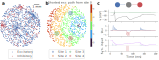
\includegraphics[width=\linewidth]{fig1}
    \caption{%
        Model and paradigm.
        \textbf{A} Membrane and synaptic dynamics of a neuron innervated by an excitatory and an inhibitory neuron firing pre-determined spikes, illustrated above the plots. The excitatory connection has weight $w = 3$ for demonstration purposes only; a single connection with $w = 1$ is normally unable to evoke postsynaptic firing. Top: Inputs to the (post-)synaptic conductances $g_e$ and $g_i$ (vertical bars), and the STD depression variable $x_{Exc}$ of the excitatory presynaptic neuron (dashed line). Note that excitatory inputs are equal to $U x_{Exc} w$ as per \EQ{gsyn}. Middle: Excitatory and inhibitory synaptic conductances ($g_e$ and $g_i$, respectively). Bottom: Membrane voltage, firing threshold baseline (gray) and adaptive threshold, demonstrating TA in the excitatory postsynaptic neuron.
        \textbf{B} Sample network layout, showing the spatial location of excitatory and inhibitory neurons, and all outgoing synaptic connections from two neurons of each type.
        \textbf{C} Distance from stimulation site 1 in terms of minimum number of excitatory synapses. Stimulation is provided to the 10 neurons nearest to the center of each of 5 stimulation sites (large circles), which are regularly spaced on a circle with a radius of 2.5 mm.
        \textbf{D} Illustration of the stimulation paradigm. Each marker represents a stimulation, with the stimulus identity indicated by color. The target stimulus (A) is represented as solid red, and non-target stimuli are represented with faded colors. Three randomized sequences were presented, containing 80\% A and 20\% B (\std{}), 20\% A and 80\% B (\dev{}), and 20\% of each of 5 stimuli, including A and B (\msc{}). Note that, while the onset asynchrony of 500 ms is represented faithfully, the horizontal extent of the stimulation markers has no meaning; stimuli were presented instantaneously rather than over an extended period.
    }
    \label{fig:1}
\end{figure}

\FIG{1}A shows the internal and presynaptic dynamics of an excitatory neuron in a contrived example for the purpose of illustration. The model was implemented in Brian2 \citep{Stimberg2019-tc}, accelerated with Brian2GeNN \citep{Stimberg2020-go}, and simulated with an integration time step of 1~ms. Synaptic delay was not modeled explicitly, but spikes were delivered, and voltages reset, in the time step following spike emission. We simulated neurons without any stochasticity in either their inputs or their parameters, other than network structure (described below), in order to ensure that our results were driven purely by the experimental paradigm, rather than any model-internal sources of noise.

800 excitatory and 200 inhibitory neurons were placed randomly in a two-dimensional circular space with a radius of 4~mm, and formed synapses of weight $w = 1$ with 50 randomly selected postsynaptic partners within a range of 2~mm (excitatory) or 1~mm (inhibitory), reflecting the notion that excitatory neurons project over longer distances, while inhibitory neurons mainly connect to their local neighborhood. Connectivity and weights remained fixed throughout. Stimulation sites were evenly distributed 2.5~mm from the center of the dish, and stimulation delivered a one-time increase in $g_e$ to the 10 closest neurons, sufficient to trigger 2-3 spikes each. \FIG{1}B shows a representative example of the resulting network structure. In \FIG{1}C, we show the distance from the neurons stimulated at site 1 to each neuron in this network, in terms of the minimum number of excitatory synapses that need to be traversed to reach the target, in order to give an intuition for how activity may spread. Networks were pseudo-randomly generated according to the above scheme and screened for minimal stimulus response: Networks where fewer than 500 neurons responded to stimulation at any of the five sites after full recovery were discarded. In total, 30 networks were used for the experiments described below.

\subsection{Paradigm}\label{sec:paradigm}

To investigate deviance detection, we used a classical oddball paradigm as illustrated in \FIG{1}D, presenting a total of 500 stimuli at regular intervals of 500~ms. Target stimuli (labeled ``A'' or ``target'' hereafter) and distractor stimuli (labeled B to E) were presented in three randomized sequences: The ``standard'' sequence (\std{}), consisting of 400 presentations of A and 100 presentations of B; the ``deviant'' sequence (\dev{}) with 100 A and 400 B, and the many-standards control sequence (\msc{}) with 100 presentations of each of the stimuli A through E. In this way, A is presented as the predominant and therefore expected stimulus (\std{}), as an infrequent violation of an expectation (of B, \dev{}), and, to control for pure adaptation effects, as an equally infrequent stimulus with no strong expectation of any particular input (\msc{}).

In each network, we simulated oddball sequences with two A/B stimulus pairs (sites 1 and 2 in one pair, and sites 3 and 5 in the other pair), where each stimulus site in a pair was used once as target (A) and once as non-target (B), and a single \msc{} sequence involving all sites. Networks were reset to a fully recovered state between sequence presentations to guarantee their independence. This yielded 4 complete data sets per network, or a total of 120 data sets across all networks.

In order to disentangle the effects of STD and TA, we ran all simulations in four conditions: Without any short-term plasticity, with either TA only or STD only, and with both STD and TA (labeled STD+TA in the following, and corresponding to the full model as described above). To turn off STD, we replaced \EQ{xsyn} with a constant $x = 1$, but retained the scaling of inputs to $g_e$ with $U$ in \EQ{gsyn}. This corresponds to immediate recovery ($\tau_x = 0$) and was done to maintain the magnitude of the excitatory postsynaptic potential (EPSP) in the recovered state regardless of whether STD was turned on or off. To turn off TA, we replaced \EQ{TA} with a constant $V_{\theta} = \theta_0$, making the firing threshold completely unadaptive.

\subsection{Sample network}\label{sec:sample}

We present most of our analysis at two levels: We first detail the processes leading to deviance detection on a sample network, then confirm the highlighted trends statistically with reference to the full set of 120 networks and stimulus assignments. The sample network was chosen to be roughly representative of the population as follows: We assessed each network's average response to stimulation with A and B in the \msc{} sequence and calculated z-scores with respect to the population. We considered only networks whose absolute z-score was less than 1 for both A and B responses, then hand-picked a sample network and stimulus assignment that exhibited both an increased deviance detection index (see \EQ{ddi} below) in STD+TA over TA only, and greater \msc{} than \std{} responses in both STD+TA and TA only conditions.

\subsection{Notation}\label{sec:notation}

Throughout this paper, we refer to three main quantities of interest: the stimulus response magnitude $\R{}{}$, the threshold adaptation value $\T{}{}$, and the short-term depression value $\D{}{}$. We define the response $\R{}{}$ as the mean number of spikes fired across all indicated trials (see below), i.e., the average trial response. We define $\T{}{}$ as the mean across trials of $\theta(t=0)$, i.e., the average TA voltage at the beginning of trials, immediately before stimulation. Lastly, the related STD quantity $\D{}{}$ will be introduced later in \EQ{D}.

We employ sub- and superscripts to indicate the precise quantity as follows, using $\R{}{}$ for illustration: $\R[seq]{X}{p}$ refers to the response of neuron(s) $p$, averaged across all trials of type $X$ in the sequence $seq$. We use $p$ to either identify individual neurons (e.g., $i$ or $j$), or a subpopulation (e.g., $exc$) or the whole network (no index), in which case the designated quantity is the median of the individual quantities $\R[seq]{X}{i}$ across the indicated set of neurons. The trial type $X$ is either $A$ or $B$, referring to trials with stimulation at these sites, or $N$, indicating all \textit{n}on-target trials B through E. Finally, we use the notation $\Delta \R{}{}$ to refer to the sequence contrast $\R[dev]{}{} - \R[msc]{}{}$, and $\mean{\R{}{p}}$ to indicate the mean, rather than median, of the individual quantities in a population $p$.

For disambiguation, note that the quantity $\T{X}{i}$, regardless of sub- and superscripts, is always in bold math font, whereas the Wilcoxon statistic T is typeset in normal font.

\section{Results}\label{sec:results}

\subsection{Deviance detection}\label{sec:dd}

We define deviance detection as a network's ability to pick out unexpected inputs from an otherwise homogeneous or otherwise unsurprising stream of inputs. Following related research \citep{Kubota2021-dx,Harms2014-ah,Jacobsen2001-sc}, we were careful to exclude effects due to stimulus identity (i.e., avoiding direct comparisons between different stimuli) or due to adaptation to frequent stimulus presentation (i.e., avoiding direct comparisons of A in the \dev{} sequence to A in the \std{} sequence). In other words, we used the \msc{} sequence as a neutral baseline where the target stimulus was presented no more often than in the \dev{} sequence, but no expectation of a competing stimulus B could be formed. To quantify deviance detection, we compared the mean number of spikes fired per neuron in response to target stimulus A in the \dev{} and \msc{} sequences, denoted as $\mean{\R[dev]{A}{}}$ and $\mean{\R[msc]{A}{}}$, respectively, and define a deviance detection index (DDI) as
\begin{equation}
    DDI = \frac{\mean{\R[dev]{A}{}} - \mean{\R[msc]{A}{}}}{\mean{\R[dev]{A}{}} + \mean{\R[msc]{A}{}}} \label{eq:ddi}
\end{equation}

\begin{figure}
    \includegraphics[width=\linewidth]{fig2}
    \caption{%
        Deviance detection in our model.
        \textbf{A} Sample network target response intensity by trial type. Each horizontal line of the plot summarizes the network response in one target trial in terms of spikes per integration time step. Target trials are taken from the \std{} (400), \msc{} (100), and \dev{} (100) sequences, and sorted by sequence time (earliest trials are at the bottom of each section).
        \textbf{B} Response summary, showing average network-wide spike counts in target trials in each sequence. The underlying data are the same as in panel A. Note how the \dev{} response is very large, followed by an intermediate \msc{} response and a low \std{} response.
        \textbf{C} Mean response sizes $\mean{\R[dev]{A}{}}$ and $\mean{\R[std]{A}{}}$, normalized by $\mean{\R[msc]{A}{}}$, across networks and stimuli (n = 120). In this and later boxplots, the median is indicated with an orange line, notches indicate the 95\% confidence interval for the median calculated by bootstrap with 10000 iterations, boxes indicate the inter-quartile range (IQR), whiskers extend to 1.5 times the IQR or to the data extrema, whichever is less, and fliers indicate individual data points beyond the whisker end points.
        \textbf{D} Deviance detection indices (DDI, see Equation {eq:ddi}) across networks and stimuli.
    }
    \label{fig:2}
\end{figure}

To show that our model is capable of deviance detection, we first show the responses of the sample network in all sequences (\dev{}, \msc{}, and \std{}) in \FIG{2}A. Here, each row corresponds to one trial, aligned to stimulus input at t = 0, with the number of spikes in each millisecond bin indicated by color. All responses share an early activity pattern, which derives from the stimulated neurons and their immediate postsynaptic targets, but differences soon start to emerge. The \dev{} sequence responses, shown at the top of the plot, exhibit a clear peak in activity around 15 ms after stimulation. The \std{} sequence responses show a later, more diffuse activity peak around 20 ms, and the \msc{} sequence responses lack any obvious activity cluster. We sum these patterns up in \FIG{2}B, where we show the mean network activity, in terms of spikes per millisecond bin, across trials of each type. Clearly, the target response in the \dev{} sequence is greater than either the \msc{} or the \std{} response.

We could readily identify similar patterns emerging across most networks and stimulus assignments. To show that deviance detection is robust to network and stimulus identity, we calculated the average spike count per neuron per target trial for each network and stimulus assignment, and compared these across sequences. \FIG{2}C shows a summary of the average \dev{} and \std{} response sizes, normalized by the response in the \msc{} sequence. The data clearly confirmed that \dev{} responses were larger than \msc{} (T = 6.38e+03, p = 2.75e-13; one-sided Wilcoxon signed-rank test, n = 120), and \std{} responses smaller (T = 687, p = 6.42e-15). Accordingly, the DDI (\FIG{2}D) was positive in most networks (T = 5.97e+03, p = 4.75e-10, median 0.114). This shows that our model was well behaved and suitable for an investigation of deviance detection.

\begin{figure}
    \includegraphics[width=\linewidth]{fig3}
    \caption{%
        Deviance detection under model ablation.
        \textbf{A} Sample network responses to target stimulation, with the deviance detection index in each instance noted in the plot titles. Lines show the average (trial mean +- SEM, left axis) network-wide spike counts in target trials in each sequence. Boxes summarize the spike count totals per trial (right axis), the means of which form the basis for index calculations (see panel C). Note the different axis scaling on the top row (without TA) and the bottom row (with TA).
        \textbf{B} Deviance detection indices across networks and stimuli. Asterisks indicate data greater than 0, established with a Wilcoxon signed-rank test at a significance level 0.05. See main text for detailed statistics.
    }
    \label{fig:3}
\end{figure}

Having confirmed the presence of deviance detection in our model, we turned to an ablation approach to try to identify how the two short-term plasticity mechanisms in the model, STD and TA, enabled the networks to learn relevant regularities. \FIG{3}A shows the responses to target stimulation of the sample network under ablation. With no plasticity, the responses are indistinguishable between sequences, yielding a DDI of 0, and indicating that stimulation did not have any long-lasting effects in membrane voltage or synaptic conductance. With STD only, the response in the \dev{} sequence developed earlier and very slightly larger, yielding a DDI of 0.03. With TA only, the response became noticeably smaller, but the sequences became readily distinguishable, with high \dev{}, intermediate \msc{}, and low \std{} responses, yielding a DDI of 0.19. Finally, in the full model, the \dev{} response stood out more clearly, leaving much smaller \msc{} and \std{} responses and yielding a DDI of 0.4.

Finally, across networks and stimuli, the DDI (\FIG{3}C) was exactly 0 as expected in the ablation with no plasticity, not significantly different from 0 with STD only (T = 3.2e+03, p = 0.262, median -2.1e-04; two-sided Wilcoxon, n = 120), but clearly positive for TA only (T = 5.85e+03, p = 3.1e-09, median 0.077; one-sided Wilcoxon, n = 120) and the full model (T = 5.97e+03, p = 4.75e-10, median 0.114). To our surprise, the DDI of the full model was significantly greater than that of either plasticity mechanism alone (STD: T = 6.1e+03, p = 4.95e-11; TA: T = 4.87e+03, p = 0.000604), and greater too than the sum of the DDI values across both STD only and TA only models (T = 5.12e+03, p = 4.52e-05). This suggests that TA and STD act not as independent mechanisms in this paradigm, but rather interact constructively to enhance the network's ability to encode input regularities.

In the following, we will first build an understanding of how TA leads to deviance detection when acting alone, i.e., in the ablated TA only model, working backwards from the increased target response in \dev{}, identifying and tracing causal factors step by step. Then, we will build on this understanding to elucidate how the addition of STD, which was shown above to be ineffective for deviance detection on its own, can lead to an increased deviant response in the full model.

\subsection{The role of TA in deviance detection}\label{sec:ta}

To understand why the same stimulus A evoked a higher response in \dev{} than in \msc{} with TA only, we first compared the average responses in the two sequences, sorting neurons by their response onset to permit a high-resolution view of the stimulus response as it propagates through the network. As shown in \FIG{4}A (left and middle), we found that the response developed in a qualitatively similar fashion in both sequences. The contrast (right) revealed a clear increase in \dev{} spikes, particularly in the later parts of the response, as shown by the predominance of orange areas, which indicate higher \dev{} activity. Since the stimulus was identical in both sequences, and TA was the only plasticity mechanism in play, these differences had to be due to (1) different firing thresholds, and/or (2) different synaptic currents as a consequence of different prior activity within the trial.

\begin{figure}
    \includegraphics[width=\linewidth]{fig4}
    \caption{%
        Responses to \dev{} target trials are larger due to lower initial $\theta$.
        \textbf{A} Post-stimulus spike histogram across target trials in the sample network, showing trial time along the horizontal axis, and neurons along the vertical, sorted by the time of the first recorded spike across all trials and sequences. Left and middle column, target trials in the \dev{} sequence and \msc{} sequence, respectively; right column, contrast between these two.
        \textbf{B} Target trial average of the threshold adaptation voltage $\theta$, with neuron order and columns as in panel A.
        \textbf{C} Target trial average of the membrane potential $V_m$, with neuron order and columns as in panel A. The first 10 ms of the neurons under direct stimulation are masked out to avoid saturation of the colormap.
        \textbf{D} Relationship across excitatory neurons of the sample network between the contrast (dev - msc) in $\theta$ at the start of target trials ($\Delta \T{A}{i}$) and the contrast in the average number of spikes fired in target trials ($\Delta \R{A}{i}$), and associated linear regression.
        \textbf{E} $\Delta \T{A}{exc}$ across networks and stimuli, plotted against the Pearson correlation coefficients $\rho$ of the relationship shown in the previous panel ($\Delta \T{A}{i}$ vs $\Delta \R{A}{i}$ across excitatory neurons). Each marker corresponds to one network and target stimulus. Red markers indicate a significant negative correlation (one-sided Wald test, significance level 0.05). Inset histograms show the distribution of the corresponding values, with orange portions indicating the 95\% confidence interval of the median, calculated by bootstrap with 10000 iterations.
        \textbf{F} In the sample network, contribution of the contrast in $\theta$ and $V_m$ to bins with increased firing in \dev{} (i.e., positive/red bins in the spike probability contrast, panel A), weighted by that same contrast.
        \textbf{G} Contribution of $\theta$ relative to the sum of the absolute values of the weighted contributions in panel F.
        \textbf{H} Relative contribution of $\theta$ across networks and stimuli, showing median (solid line) and inter-quartile range (shaded area).
    }
    \label{fig:4}
    % 
    \figsupp[The equivalent figure in the full model with both TA and STD.]{%
        The equivalent of \FIG{4} in the full model with both TA and STD.
        \textbf{A} Post-stimulus spike histogram across target trials in the sample network, showing trial time along the horizontal axis, and neurons along the vertical, sorted by the time of the first recorded spike across all trials and sequences. Left and middle column, target trials in the \dev{} sequence and \msc{} sequence, respectively; right column, contrast between these two.
        \textbf{B} Target trial average of the threshold adaptation voltage $\theta$, with neuron order and columns as in panel A.
        \textbf{C} Target trial average of the membrane potential $V_m$, with neuron order and columns as in panel A. The first 10 ms of the neurons under direct stimulation are masked out to avoid saturation of the colormap.
        \textbf{D} Relationship across excitatory neurons of the sample network between the contrast (dev - msc) in $\theta$ at the start of target trials ($\Delta \T{A}{i}$) and the contrast in the average number of spikes fired in target trials ($\Delta \R{A}{i}$), and associated linear regression.
        \textbf{E} $\Delta \T{A}{exc}$ across networks and stimuli, plotted against the Pearson correlation coefficients $\rho$ of the relationship shown in the previous panel ($\Delta \T{A}{i}$ vs $\Delta \R{A}{i}$ across excitatory neurons). Each marker corresponds to one network and target stimulus. Red markers indicate a significant negative correlation (one-sided Wald test, significance level 0.05). Inset histograms show the distribution of the corresponding values, with orange portions indicating the 95\% confidence interval of the median, calculated by bootstrap with 10000 iterations.
        \textbf{F} In the sample network, contribution of the contrast in $\theta$ and $V_m$ to bins with increased firing in \dev{} (i.e., positive/red bins in the spike probability contrast, panel A), weighted by that same contrast.
        \textbf{G} Contribution of $\theta$ relative to the sum of the absolute values of the weighted contributions in panel F.
        \textbf{H} Relative contribution of $\theta$ across networks and stimuli, showing median (solid line) and inter-quartile range (shaded area).
    }
    {\includegraphics[width=\linewidth]{fig4-withSTD}}\label{figsupp:withSTD}
\end{figure}

We quantified the former with the strength of adaptation $\theta$ (\EQ{TA}), i.e., the amount by which the firing threshold was raised due to TA. As shown in \FIG{4}B, there was a clear and widespread lowering of thresholds at the start of target \dev{} trials relative to \msc{}, visible both in the raw data (left and middle panels) and in the contrast (right panel, early blue portions). On the other hand, once the bulk of activity had occurred, many neurons showed higher thresholds in \dev{} (right panel, later orange portions), since they spiked more often. Finally, note that inhibitory neurons, which were modeled without TA, naturally showed no difference in $\theta$, leading to numerous horizontal breaks in the plot.

To assess the difference in synaptic currents in a way that allowed direct comparison to $\theta$, we refer to the membrane voltage $V_m$, which is largely independent from and complementary to the firing threshold, and driven mostly by presynaptic inputs, resets after spikes notwithstanding. As the immediate cause of neuronal spiking, the overall pattern of $V_m$ (\FIG{4}C) largely reflected that seen in spiking activity. The contrast (right panel) shows not only a notable relative increase in membrane voltages in \dev{} around the typical response time (note the orange band running along the response front), but also an increased hyperpolarization starting immediately after due to post-spike resets.

Based on these measures, we then asked why there were more spikes in \dev{} trials. We first focused on the contribution of $\theta$ alone to confirm that thresholds are lower in \dev{}, and that this reduction in thresholds causes increased firing. We quantified the contrast in $\theta$ at the start of target trials as $\Delta \T{A}{i} = \T[dev]{A}{i} - \T[msc]{A}{i}$, where $\T{}{i} = \theta_i(t=0)$, corresponding to the leftmost datapoints of the contrast histogram in \FIG{4}B, and correlated this with the target trial response size contrast $\Delta \R{A}{i}$ across excitatory neurons. In the sample network (\FIG{4}D), we found that thresholds were clearly lower in \dev{} than \msc{} (T = 2.69e+04, p = 1.58e-92, median = -0.166 mV; one-sided Wilcoxon, n = 800 excitatory neurons), and that this decrease was accompanied by an increase in the target trial response at the level of individual neurons (Pearson's $\rho$ = -0.424, p = 1.6e-36; one-sided Wald test, n = 800). As shown in \FIG{4}E, this relationship held across networks and stimuli: The median of $\T{A}{i}$ among excitatory neurons was lower in \dev{} than \msc{} ($\Delta \T{A}{exc} < 0$: T = 514, p = 1.67e-16, grand median = -0.094 mV; one-sided Wilcoxon, n = 120), indicating that networks were less adapted during oddball sequences. In addition, the correlation across excitatory neurons between $\Delta \T{A}{i}$ and $\Delta \R{A}{i}$ was almost universally negative (T = 40, p = 2.68e-21, median = -0.357). This indicates that neurons with a greater decrease in $\T[dev]{A}{i}$ tended to show a greater increase in their response to target stimuli.

Yet, as we saw in \FIG{4}C, the membrane voltages also differed between the two sequences. In order to assess the relative contribution of $\theta$ to the increased \dev{} response, we chose to focus exclusively on time points with higher firing probability in the \dev{} sequence, discarding data points with equal or lower firing probability relative to the \msc{} sequence. We then weighted the remaining contrasts in $\theta$ and $V_m$ by the magnitude of the response difference and summed across neurons. The resulting time courses, shown in \FIG{4}F, show how much these two measures contributed to the increased \dev{} response. While thresholds were slightly lowered throughout the response, the membrane potential was dramatically increased. In relative terms (\FIG{4}G), $\theta$ constituted a major driver of increased firing right at the onset of the response, as well as briefly towards the end of the response. A similar pattern emerged across networks and stimuli, as shown in \FIG{4}H. Here, only the initial response was driven mainly by $\theta$, while later differences were largely explained by differences in $V_m$, leading to a relative TA contribution of less than 20\% on average. This indicates that adaptation initiated and dominated the increase in firing at the start of trials, whereas the late response was enlarged primarily as a result of increased presynaptic excitation.

Having established that the increased response to A in \dev{} trials was driven by lower thresholds before stimulation, we next turned to the cause of this reduction. A priori, since threshold adaptation is a direct reflection of activity, and since the response to target trials was larger in \dev{} than in \msc{}, the lower thresholds in \dev{} must have been caused by lower activity in non-target trials, i.e., by lower responses to B in \dev{} than to B through E in \msc{}. Yet, since activity was modulated by thresholds as shown above, and since the dev sequence was random, implying that $\T[dev]{A}{} \approx \T[dev]{B}{}$, we might expect the lowered thresholds in \dev{} to yield not only higher target responses, but also higher non-target responses. To resolve this apparent paradox, we will turn to an analysis of the spatial arrangement of activity and adaptation.

\begin{figure}
    \includegraphics[width=\linewidth]{fig-thresholds-follow-std}
    \caption{%
        Lower thresholds in \dev{} are a consequence of lower \dev{} non-target response magnitude.
        \textbf{A} $\T{A}{i}$ in the sample network, with each neuron shown in its spatial location. Left and middle column, raw averages in the \dev{} sequence ($\T[dev]{A}{i}$) and \msc{} sequence ($\T[msc]{A}{i}$), respectively; right column, contrast between these two ($\Delta \T{A}{i}$). A and B stimulus locations are highlighted in the left plot; see \FIG{1} for the locations of the remaining stimuli used in the \msc{} sequence.
        \textbf{B} Average response (in spikes per trial) to non-target trials ($\R{N}{i}$, with $N$ meaning B in \dev{}, and B, C, D, and E in \msc{}). Columns are arranged as in panel A.
        \textbf{C} Relationship across excitatory neurons of the sample network between $\Delta \R{N}{i}$ and $\Delta \T{A}{i}$, and associated linear regression.
        \textbf{D} $\Delta \R{N}{exc}$ across networks and stimuli, plotted against the Pearson correlation coefficients $\rho$ of the relationship shown in the previous panel ($\Delta \R{N}{i}$ vs $\Delta \T{A}{i}$ across excitatory neurons). Each marker corresponds to one network and target stimulus. Red markers indicate a significant positive correlation (one-sided Wald test, significance level 0.05). Inset histograms show the distribution of the corresponding values, with orange portions indicating the 95\% confidence interval of the median, calculated by bootstrap with 10000 iterations.
    }
    \label{fig:thresholds-follow-std}
    % 
    \figsupp[The equivalent figure in the full model with both TA and STD.]{%
        The equivalent of \FIG{thresholds-follow-std} in the full model with both TA and STD.
        \textbf{A} $\T{A}{i}$ in the sample network, with each neuron shown in its spatial location. Left and middle column, raw averages in the \dev{} sequence ($\T[dev]{A}{i}$) and \msc{} sequence ($\T[msc]{A}{i}$), respectively; right column, contrast between these two ($\Delta \T{A}{i}$). A and B stimulus locations are highlighted in the left plot; see \FIG{1} for the locations of the remaining stimuli used in the \msc{} sequence.
        \textbf{B} Average response (in spikes per trial) to non-target trials ($\R{N}{i}$, with $N$ meaning B in \dev{}, and B, C, D, and E in \msc{}). Columns are arranged as in panel A.
        \textbf{C} Relationship across excitatory neurons of the sample network between $\Delta \R{N}{i}$ and $\Delta \T{A}{i}$, and associated linear regression.
        \textbf{D} $\Delta \R{N}{exc}$ across networks and stimuli, plotted against the Pearson correlation coefficients $\rho$ of the relationship shown in the previous panel ($\Delta \R{N}{i}$ vs $\Delta \T{A}{i}$ across excitatory neurons). Each marker corresponds to one network and target stimulus. Red markers indicate a significant positive correlation (one-sided Wald test, significance level 0.05). Inset histograms show the distribution of the corresponding values, with orange portions indicating the 95\% confidence interval of the median, calculated by bootstrap with 10000 iterations.
    }
    {\includegraphics[width=\linewidth]{fig-thresholds-follow-std-withSTD}}\label{figsupp:withSTD}
\end{figure}

First, we mapped the average value of $\theta$ at the start of target trials, $\T{A}{i}$, to the spatial location of the neurons, as shown in \FIG{thresholds-follow-std}A. In the \msc{} sequence, $\T[msc]{A}{i}$ was roughly evenly distributed across the network, consistent with the random, distributed nature of stimulation. Conversely, in the \dev{} sequence, a small number of neurons near the non-target stimulation site (B) were strongly adapted, whereas most of the network was less adapted, consistent with the data shown above.

Visualizing the likely cause of this difference, the non-target responses, in the same fashion (\FIG{thresholds-follow-std}B), we see that the pattern of activity in non-target trials, constituting 80\% of all trials, closely matched that of the thresholds, as expected. Notably, although the comparison is between 400 B trials in \dev{}, and only 100 B trials (alongside the same number of C, D and E trials) in \msc{}, only a small handful of neurons responded more to non-target stimulation in \dev{}, most of these very close to the stimulation site of B.

Correlating $\Delta \R{N}{i}$ with $\Delta \T{A}{i}$ across excitatory neurons (\FIG{thresholds-follow-std}C), we found that the reduced non-target response magnitude in \dev{} almost perfectly predicted the resulting reduction in TA levels before target stimuli (Pearson's $\rho$ = 0.99).
This finding held across networks and stimuli, as shown in \FIG{thresholds-follow-std}D, with a median correlation coefficient of 0.99 and a consistent reduction in the median non-target response $\R{N}{}$ between \msc{} and \dev{} sequences (T = 525, p = 2.12e-16, median = -0.094; one-sided Wilcoxon, n = 120), clearly validating our notion that the reduced non-target trial response was the primary driver of lower TA, which we showed above to be responsible for the higher target response.

Finally, we examined the cause of the reduced response in non-target trials. Going from the \msc{} sequence to the \dev{} sequence, two things change: Firstly, stimulations with non-target C, D and E are replaced with B, which would cause different responses even in the absence of adaptation. Secondly, the resulting  frequent presentation of B changes TA values, likely causing adaptation to B and thereby decreasing the average response. We hypothesized that this adaptation is mediated by a small subset of neurons that (1) responds very quickly and rather strongly to stimulation in B (and therefore more to non-target stimuli in \dev{} than \msc{}), and (2) has increased TA levels as a result, reducing the response of the remaining downstream neurons in the same way as demonstrated in reverse in \FIG{4}.

\begin{figure}
    \includegraphics[width=\linewidth]{fig-early-adaptation}
    \caption{%
        Dev non-target responses are reduced due to adaptation in early responders to B.
        \textbf{A} The sample network, colored by latency rank, i.e. the rank order of the time to first spike in response to stimulation at site B in any sequence. The response develops asymmetrically due to structural properties, not due to interactions with A. Note that non-responding neurons are ranked last and appear dark blue.
        \textbf{B} Relationship across excitatory neurons of the sample network between $\Delta \R{N}{i}$ and $\Delta \T{B}{i}$, and associated linear regression. Neurons are colored by latency rank as in panel A. Additionally, excitatory neurons among the earliest 100 responders are shown in the left plot, while later responders are shown in the right plot. Inset histograms show the distributions of the plotted values, with the confidence intervals of their medians, calculated by bootstrap with 10000 iterations, in darker color.
        \textbf{C} Median non-target response contrast $\Delta \R{N}{}$ among the first 100 neurons to respond to stimulation in B, labeled ``early'', and among the later neurons, labeled ``late'', across networks and stimuli.
        \textbf{D} Median contrast in $\T{B}{}$ among the early and late neurons, respectively, across networks and stimuli.
        \textbf{E} Relationship across networks and stimuli between $\Delta \T{B}{early}$ and $\Delta \R{B}{}$, and associated linear regression.
    }
    \label{fig:early-adaptation}
    % 
    \figsupp[The equivalent figure in the full model with both TA and STD.]{%
        The equivalent of \FIG{early-adaptation} in the full model with both TA and STD.
        \textbf{A} The sample network, colored by latency rank, i.e. the rank order of the time to first spike in response to stimulation at site B in any sequence. The response develops asymmetrically due to structural properties, not due to interactions with A. Note that non-responding neurons are ranked last and appear dark blue.
        \textbf{B} Relationship across excitatory neurons of the sample network between $\Delta \R{N}{i}$ and $\Delta \T{B}{i}$, and associated linear regression. Neurons are colored by latency rank as in panel A. Additionally, excitatory neurons among the earliest 100 responders are shown in the left plot, while later responders are shown in the right plot. Inset histograms show the distributions of the plotted values, with the confidence intervals of their medians, calculated by bootstrap with 10000 iterations, in darker color.
        \textbf{C} Median non-target response contrast $\Delta \R{N}{}$ among the first 100 neurons to respond to stimulation in B, labeled ``early'', and among the later neurons, labeled ``late'', across networks and stimuli.
        \textbf{D} Median contrast in $\T{B}{}$ among the early and late neurons, respectively, across networks and stimuli.
        \textbf{E} Relationship across networks and stimuli between $\Delta \T{B}{early}$ and $\Delta \R{B}{}$, and associated linear regression.
    }
    {\includegraphics[width=\linewidth]{fig-early-adaptation-withSTD}}\label{figsupp:withSTD}
\end{figure}

To show this, we sought to isolate this subset of early responders to B. In a given network and stimulus assignment, we ranked each neuron by the minimum response time (i.e., time to first spike) across B trials in all sequences. The ranking in the sample network is shown in \FIG{early-adaptation}A. We found that the response developed in an approximately radial pattern, spreading outward in all directions from the stimulus site. We did notice that the early response appeared to gravitate towards the stimulus site for A, but confirmed that this was the case in all sequences separately, indicating a structural rather than dynamic cause (data not shown). We then notionally split the network into an early portion, containing the first 100 neurons to respond to B, and a late portion, containing the remaining 900 neurons. In \FIG{early-adaptation}B, we related the non-target response contrast, $\Delta \R{N}{i}$, to the contrast in $\theta$ at the start of B trials, $\Delta \T{B}{i}$. Across excitatory neurons, a strong linear relationship (Pearson's $\rho$ = 0.993, n = 800) echoed the related finding in \FIG{thresholds-follow-std}C, where we correlated $\Delta \R{N}{i}$ to $\Delta \T{A}{i}$. As the color coding and inset histograms show, however, there was a clear separation between the early and late portions of the network, with many early neurons (red, left plot) increasing their response in the \dev{} sequence, while the response of the later portion of the network (blue, right plot) decreased. Correspondingly, the TA levels of the early portion also tended to increase, in clear contrast to the later portion.

Across networks and stimuli, we found even stronger evidence that the early portion of the network drove adaptation to B. We first confirmed that $\Delta \R{N}{i}$ and $\Delta \T{B}{i}$ were robustly positively correlated (median Pearson's $\rho$ 0.992: T = 7.26e+03, p = 9.86e-22; one-sided Wilcoxon, n = 120). In each network, we then identified the early and late portions with respect to stimulation in B and quantified the median non-target response contrast ($\Delta \R{N}{}$, \FIG{early-adaptation}C) and the median contrast in $\T{B}{}$ ($\Delta \T{B}{}$, \FIG{early-adaptation}D) within these two portions. We found that the response in the early portion was consistently greater in \dev{} than \msc{} ($\Delta \R{B}{early} > 0$: T = 6.98e+03, p = 8.48e-19), unlike the late portion, which decreased ($\Delta \R{B}{late} < 0$: T = 295, p = 1.23e-18; see also \FIG{thresholds-follow-std}D). $\Delta \T{B}{}$ followed the same pattern, with the early portion exhibiting stronger TA in \dev{} (T = 4.63e+03, p = 2.21e-17), while the late portion was instead more recovered (T = 26, p = 2.97e-17).

Finally, to show that high $\T[dev]{B}{early}$ was causal in reducing the response to B, we correlated the median contrast in $\T{B}{}$ among the early portion, $\Delta \T{B}{early}$, with the network-wide median contrast of the response to B, $\Delta \R{B}{}$, as shown in \FIG{early-adaptation}E. Across networks and stimuli, we found a strong negative correlation ($\rho$ = -0.587, p = 9.56e-13, Wald test, n = 120), indicating that greater TA in the neurons responding early was indeed predictive of a lowered response to B in the overall network.

To sum up, we showed in \FIG{4} that lower $\T[dev]{A}{}$ in the portion of the network responding earliest to A played an important role in increasing the overall response to A. Here, we showed that the neurons responding earliest to B exhibited higher $\T[dev]{B}{}$, which analogously reduced the response of the network as a whole to B. We also showed that this increase in $\T[dev]{B}{early}$ was a consequence of an increased response to non-target stimulation in the early portion, or in other words, a direct consequence of the more frequent presentation of B.

Thus, we have finally traced the greater response to A in the \dev{} sequence to its roots and revealed two complementary roles of TA: The frequent presentation of non-target stimulus B in the \dev{} sequence and concomitant increased activity in a subset of neurons responding early to B causes \emph{local suppression} by TA in this subset, leading to smaller network responses. By contrast, stimuli in the \msc{} sequence are presented more sporadically, allowing local suppression to decay, thus leading to larger network responses. This difference in non-target response sizes -- small in \dev{}, large in \msc{} -- is then reflected in network-wide \emph{global suppression}, such that the network is more excitable to stimulation with A (or other infrequent inputs) in the \dev{} sequence than in the control context.

\subsection{The role of STD in deviance detection}\label{sec:std}

As noted previously, STD alone exerted no deviance detection effect, but its addition did enhance the deviance detection effect established by TA. To understand the basis of this apparent synergy, we contrasted the TA only condition examined in the previous section against the same networks evaluated in the full model with both TA and STD. On average, adding STD caused a reduction in response magnitude across the board, as we would expect from a depression mechanism (\FIG{addingSTD}A). However, this reduction was not uniform: Target responses $\mean{\R{A}{}}$ were reduced most in the \std{} sequence (more than \msc{}: T = 2.99e+03, p = 0.0474; one-sided Wilcoxon, n = 120), and least in the \dev{} sequence (less than \msc{}: T = 2.66e+03, p = 0.00554).

\begin{figure}
    \includegraphics[width=\linewidth]{fig-addingSTD}
    \caption{%
        Adding STD to the model slightly enhances the effects of TA.
        \textbf{A} Reductions in mean response size $\mean{\R{A}{}}$ in each sequence as a consequence of adding STD to the model, across networks and stimuli.
        \textbf{B} $\Delta \R{N}{}$ (top) and $\Delta \T{B}{}$ (bottom) among early and late neurons, respectively, across networks and stimuli, in the full model with both STD and TA. Compare to \FIG{early-adaptation}C-D.
        \textbf{C} $\Delta \R{N}{exc}$ across networks and stimuli in the full model (horizontal axis) and the ablated model with TA only (vertical axis). The red line is the identity function; points above this line represent networks with greater response reduction (\dev{} - \msc{}) in the full model than in the ablated model. The subtraction of the two quantities in the box plot below shows that the non-target response tends to be reduced more in the full model.
        \textbf{D} $\Delta \R{N}{exc}$ across networks and stimuli in the full model, plotted against the corresponding Pearson coefficient of the correlation between $\Delta \R{N}{i}$ and $\Delta \T{A}{i}$ across excitatory neurons. Compare to \FIG{thresholds-follow-std}D.
        \textbf{E} $\Delta \T{A}{exc}$ across networks and stimuli in the full and ablated models, arranged as in panel C. The subtraction of the two quantities in the box plot below shows that $\T{A}{}$ tends to be reduced more in the full model.
        \textbf{F} $\Delta \T{A}{exc}$ across networks and stimuli in the full model, plotted against the corresponding Pearson coefficient of the correlation between $\Delta \T{A}{i}$ and $\Delta \R{A}{i}$ across excitatory neurons. Compare to \FIG{4}E.
        \textbf{G} $\Delta \R{A}{}$ across networks and stimuli in the full and ablated models, arranged as in panel C. The subtraction of the two quantities in the box plot below shows that the target response tends to be increased more in the full model.
    }
    \label{fig:addingSTD}
\end{figure}

To understand how STD affects deviance detection and causes this difference in response reduction, we first examined the effects of TA in the full model, following the analysis on the ablated model laid out in the previous section. Starting at the cause of the reduced response in non-target trials, we show in \FIG{addingSTD}B the full model equivalent of \FIG{early-adaptation}C-D. The contrasts (\dev{} - \msc{}) in the non-target response magnitude, $\Delta \R{N}{}$, and in the resulting $\T{B}{}$ levels both retained a clear separation between the portion of neurons responding early, which showed increased responses (T = 5.44e+03, p = 1.02e-06; one-sided Wilcoxon, n = 120) and increased TA levels (T = 3.41e+03, p = 9.51e-08), and the neurons responding later, whose response (T = 282, p = 9.19e-19) and TA levels (T = 72, p = 2.49e-17) decreased in the \dev{} sequence. Likewise, the correlation across excitatory neurons between these two contrasts remained positive (T = 7.26e+03, p = 9.86e-22) and very strong (median Pearson's $\rho$ = 0.992). This indicates that local suppression to B mediated by TA in the early responders remained a key driver of the reduced response to non-target trials.

Comparing the non-target response reductions in \FIG{addingSTD}C, we found that they were on average larger in the full model than in the ablated model (T = 4.16e+03, p = 0.0175; one-sided Wilcoxon, n = 120), with the grand medians of $\Delta \R{N}{exc}$ differing by 36\%. Based on the ablated model analysis in \FIG{thresholds-follow-std}, we expected reduced non-target responses to similarly reduce the TA levels at the start of A trials. Indeed, $\Delta \R{N}{i}$ remained tightly correlated with $\Delta \T{A}{i}$ (median Pearson's $\rho$ = 0.989), as shown in \FIG{addingSTD}D. Correspondingly, $\T[dev]{A}{exc}$ was reduced over $\T[msc]{A}{exc}$, as shown by way of their contrast in \FIG{addingSTD}E, and this too by a slightly greater amount in the full model than in the ablated model (T = 4.37e+03, p = 0.0257).

Finally, based on the ablated model analysis in \FIG{4}, we sought to confirm that lowered $\T{A}{}$ was responsible for the increased target response. As shown in \FIG{addingSTD}F, $\Delta \T{A}{exc}$ and $\Delta \R{A}{exc}$ were negatively correlated (T = 30, p = 2.09e-21, median = -0.268; one-sided Wilcoxon, n = 120), though the correlation was weaker in the full model (T = 1.67e+03, p = 1.49e-07). Despite the weaker correlation, however, the full model target response remained clearly increased in \dev{} over \msc{}, as shown in \FIG{addingSTD}G, and this increase was greater in the full model than in the ablated model (T = 1.94e+03, p = 0.000723), with the grand medians of $\Delta \R{A}{}$ differing by 94\%. This greater contrast, of course, directly reflects the greater DDI reported in \FIG{3}.

Taken together, the data indicate that, with STD added to the model, the overall chain of causality -- increased local suppression to B resulting in reduced B responses and reduced global suppression, which in turn allows greater target responses -- remained intact with only minor quantitative changes. The primary cause for the greater target response, therefore, appeared to be the smaller non-target response (\FIG{addingSTD}C), which was where we noted the first clear shift towards increased deviance detection.

This naturally raises the question of why, with the addition of STD, the non-target \dev{} response was reduced more than non-target \msc{} responses. We hypothesized that, due to its relatively short time constant, the direct effect of STD across trials was limited to repeated trials of the same stimulus, such as the frequent stimulus in oddball sequences. This would mean that STD is capable only of local suppression, reducing the non-target response in \dev{}, but not of global suppression, leaving networks with only STD unable to differentiate between \dev{} and \msc{} target trials.

We had good reasons for this assumption: Updates to the spike-triggered depression variable $x_j$ (cf. \EQ{xsyn}) would decay to a negligible $e^\frac{-1 s}{\tau_x} = 0.0013$ times the original value within two trials, making it unlikely that inputs separated by intervening trials could be ``remembered'' in the network. Conversely, the frequently presented stimulus B may have been able to lead to a build-up of depression strong enough to suppress its own response.

To show in the sample network that the model does not maintain a history beyond the most recent trial, we correlated $\R[dev]{A}{j}$ with $x_j$ at the start of later trials across excitatory neurons. We found that, while the correlation was strong and very clearly positive in the trial immediately following target (Pearson's $\rho$ = -0.984, p = 0; Wald test, n = 800), it was almost completely lost by the next trial ($\rho$ = -0.0525, p = 0.138) under the combined influence of decay and unrelated activity in the intervening trial. Similar behavior was also seen in the \msc{} sequence, as shown in \FIGSUPP[8]{correlation-decay}.

To show that STD being carried over between repeated trials was responsible for the reduction of non-target \dev{} responses relative to \msc{}, however, we needed to estimate the extent to which activity of a given neuron (or, alternatively, its membrane potential $V_m$) was affected by changes in STD. Unlike $\theta_j$, which directly affects the activity of neuron $j$, $x_j$ only exerts its effects postsynaptically. Therefore, we devised a measure $\D{}{}$ to estimate the postsynaptic impact of STD in terms of membrane potential lost, mirroring $\T{}{}$ in the sense that decreasing $V_m$ and increasing the firing threshold both increase the depolarization necessary to make a neuron fire.

A measure of STD is necessarily activity-dependent -- a postsynaptic neuron's membrane potential is driven only by presynaptic partners that fire -- so it must be calculated based on observed activity. In order to respect this notion while at the same time minimizing the influence of activity differences between sequences, we used the average response
\begin{equation}
    \Rhat{S}{j} = \frac{1}{3} (\R[dev]{S}{j} + \R[msc]{S}{j} + \R[std]{S}{j}) \label{eq:Rhat}
\end{equation}
of a neuron $j$ to a given stimulus $S$ as a measure of the presynaptic drive. Before depression, a single excitatory presynaptic spike evokes a postsynaptic potential (EPSP) peaking at approximately $k = 1.4$ mV at $V_m = V_{rest}$ (recall that $w = 1$ for all synapses), and STD linearly scales this EPSP by presynaptic $x_j$. Thus, we estimated the average peak EPSP evoked by a spike in presynaptic neuron $j$ as $\Rhat{S}{j} x_j^S k$, where we ignored added depression due to repeated spikes within a trial and instead defined $x_j^S$ as the mean depression at the start of trials. Finally, summing over presynaptic neurons, we estimated the peak EPSP lost to depression in each neuron $i$ as
\begin{equation}
    \D{S}{i} = \sum_{j \in pre} \Rhat{S}{j} (1-x_j^S) k \label{eq:D}
\end{equation}
Notice that $\D{}{}$ is measured in volts due to scaling with $k$, and is therefore roughly comparable to $\T{}{}$, albeit more approximate.

\begin{figure}
    \includegraphics[width=\linewidth]{fig-synergy}
    \caption{%
        In the full model, STD reduces \dev{} non-target and increases \dev{} target responses relative to \msc{}.
        \textbf{A} Average depression $\D{}{i}$ in target (A) trials (top row) and B trials (bottom row) in the \dev{} (left) and \msc{} sequence (center), and their contrast (right) in the sample network. The color scale is shared across columns (and between \dev{} and \msc{}) for direct comparability.
        \textbf{B} Relationship across neurons of the sample network between $\Delta \D{A}{i}$ and $\Delta \R{A}{i}$, and associated linear regression.
        \textbf{C} $\Delta \D{A}{}$ across networks and stimuli, plotted against the corresponding Pearson coefficient between $\Delta \D{A}{i}$ and $\Delta \R{A}{i}$.
        \textbf{D} $\Delta \D{B}{}$ in the first 100 neurons to respond to B, and in the remaining, late portion of the network, across networks and stimuli.
        \textbf{E} Relationship across networks and stimuli between $\Delta \D{B}{early}$ and $\Delta \R{B}{}$, and associated linear regression.
    }
    \label{fig:8}
    % 
    \figsupp[The equivalent figure in the ablated model with only STD.]{%
        The equivalent of \FIG{synergy} in the ablated model with only STD.
        \textbf{A} Average depression $\D{}{i}$ in target (A) trials (top row) and B trials (bottom row) in the \dev{} (left) and \msc{} sequence (center), and their contrast (right) in the sample network. The color scale is shared across columns (and between \dev{} and \msc{}) for direct comparability.
        \textbf{B} Relationship across neurons of the sample network between $\Delta \D{A}{i}$ and $\Delta \R{A}{i}$, and associated linear regression.
        \textbf{C} $\Delta \D{A}{}$ across networks and stimuli, plotted against the corresponding Pearson coefficient between $\Delta \D{A}{i}$ and $\Delta \R{A}{i}$.
        \textbf{D} $\Delta \D{B}{}$ in the first 100 neurons to respond to B, and in the remaining, late portion of the network, across networks and stimuli.
        \textbf{E} Relationship across networks and stimuli between $\Delta \D{B}{early}$ and $\Delta \R{B}{}$, and associated linear regression.
    }
    {\includegraphics[width=\linewidth]{fig-synergy-noTA}}\label{figsupp:noTA}
    %
    \figsupp[The STD variable $x_i$ only correlates with the activity of the immediately preceding trial.]{%
        The STD variable $x_i$ only correlates with the activity of the immediately preceding trial.
        Each marker represents the coefficient $\rho$ of the Pearson correlation between the spike counts in a target trial and the corresponding values $x_i$ at the beginning of the immediately following trial ($\Delta$ trials = 1) or after one intervening trial ($\Delta$ trials = 2). Recall that $x$ is reduced upon spiking, which implies that an effective correlation is negative. Color represents the p-value of the alternative hypothesis that $\rho < 0$. Horizontal lines indicate the median $\rho$ and p. Horizontal jitter is introduced to aid visual separability of the markers.
    }
    {\includegraphics[width=8cm]{sfig-STD-correlation-decay}}\label{figsupp:correlation-decay}
\end{figure}

As noted above, we hypothesized that STD is directly responsible only for a reduction of non-target \dev{} trials, relative to \msc{}, whereas differences between target \dev{} and \msc{} trials are not a result of STD directly. To show this, we calculated $\D{}{}$ for A and B trials and contrasted it across \dev{} and \msc{} sequences as with $\T{}{}$ before.
In \FIG{synergy}A, we see that target trials (top) experienced depression across large parts of the sample network in both sequences. The \msc{} sequence, however, clearly evoked greater depression, as borne out in the contrast $\Delta \D{A}{i}$, which was negative throughout. Conversely, depression in B trials (bottom) was spatially more clustered around the stimulation site in both sequences. In the \msc{} sequence, we can attribute the difference between A and B primarily to different response patterns due to network structure, not dynamics: The context, and thus $x$, was approximately the same, but responses to B tended not to spread out as much in this network. In the \dev{} sequence, however, the B response was limited almost exclusively to a very local patch around the stimulation site, with depression therefore similarly spatially limited. As a result, the contrast $\Delta \D{B}{i}$ was slightly reduced in the periphery, but strikingly elevated near the stimulation site, indicating greatly increased synaptic depression in \dev{}.

To show that $\D{}{}$ captures not only changes in $V_m$, by definition, but also in the resulting response, we correlated $\Delta \D{A}{i}$ with $\Delta \R{A}{i}$ across neurons of the sample network. Notice that this mirrors the correlation shown in \FIG{4} between $\Delta \T{A}{i}$ and $\Delta \R{A}{i}$. As shown in \FIG{synergy}B, the relationship was clearly negative (Pearson's $\rho$ = -0.541, p = 2.28e-77; Wald test, n = 1000), indicating that higher $\D{}{}$ causes reduced responses as expected. We confirmed this relationship across networks and stimuli, see \FIG{synergy}C, and found that greater depression in \dev{} predicted a lower response in most networks (T = 724, p = 1.37e-14; one-sided Wilcoxon, n = 120). We note that calculating this same correlation in the model with STD only yields no significantly negative dependence (T = 3.99e+03, p = 0.828; see \FIGSUPP[8]{noTA}).

Having gained a rough intuition of how individual neurons are affected by STD, we now turn to its effect on the network, working with statistics across networks and stimuli. First, in \FIG{synergy}D, we recapitulate the logic established in \FIG{early-adaptation}: Given the spatial clustering of $\D{B}{i}$, we surmised a similar local suppression effect as with TA. We found that, indeed, neurons responding early to stimulation in B showed greater depression in \dev{} than \msc{} ($\Delta \D{B}{early} > 0$: T = 7.26e+03, p = 1.01e-21; one-sided Wilcoxon, n = 120), while the late portion had slightly reduced depression ($\Delta \D{B}{late} < 0$: T = 2.24e+03, p = 0.000133). We can relate this directly to the non-target response contrasts in the early and late portions shown in \FIG{addingSTD}A, which followed a similar pattern, and take this to indicate that the increased presentation of B in \dev{} causes local synaptic suppression. % Possible concern: The relationship dXnotA ~ dD^B is not clearly established.

To show that increased local suppression by STD reduces the non-target response, we correlated $\Delta \D{B}{early}$ with $\Delta \R{B}{}$, echoing \FIG{early-adaptation}E. As we show in \FIG{synergy}E, higher $\Delta \D{B}{early}$ was clearly predictive of a lower network response ($\rho$ = -0.581, p = 1.81e-12; Wald test, n = 120). This confirms that STD-mediated local suppression played a role in reducing the non-target response in the \dev{} sequence.

Finally, given the very clear contrast in $\D{A}{i}$ in the sample network, we considered the possibility that, in the context of the full model, STD could also evoke global suppression in the \msc{} sequence, contrary to our stated hypothesis. If so, we should expect to see less $\D{A}{}$ in \dev{} than \msc{}. To confirm this, we analyzed $\Delta \D{A}{}$ across networks and stimuli and found it to be robustly negative (T = 757, p = 2.66e-14; one-sided Wilcoxon, n = 120), as can be seen in the inset histogram in \FIG{synergy}C. We conclude that there is clear evidence for greater STD-mediated global suppression in \msc{} than \dev{} in the full model.

To sum up, in the full model, STD acted in much the same way as TA, causing both a reduction in \dev{} of the response to the frequently presented non-target stimuli (lower $\R[dev]{B}{}$) by local suppression, and an increase in the response to target stimuli (higher $\R[dev]{A}{}$) by relief from global suppression, relative to \msc{}. Yet, as we showed in \FIG{addingSTD} and in the previous section, a decrease in $\R[dev]{B}{}$ also entailed lower thresholds $\T[dev]{A}{}$, which independently led to higher target responses $\R[dev]{A}{}$. Thus, adding STD to the model increased the DDI both directly, through its intrinsic effects in local and global suppression, and indirectly, by altering the pattern of TA by way of local suppression of B.

We note that the direct and indirect effects of STD on global suppression appear to be on the same order of magnitude. To see this, compare the change in $\Delta \T{A}{}$ as a result of adding STD to the model (\FIG{addingSTD}E, bottom) with the corresponding value of $\Delta \D{A}{}$ (\FIG{synergy}E), both of which are on the order of $\approx$ 0.1 mV. Conversely, notice that, since TA and STD work in similar fashion to increase the \dev{} target response, it is very plausible that TA likewise increases the effect of STD, by enhancing the STD-mediated local suppression of B and thereby increasing the contrast in STD-mediated global suppression. Thus, this synergy allows the individually weak STD to exert a significantly larger effect when paired with the stronger TA.

\subsection{Spatial basis of local suppression}

\begin{figure}
    \includegraphics[width=\linewidth]{fig-space}
    \caption{%
        Suppression acts in spatially distinguishable subpopulations.
        \textbf{A} Response size $\R{A}{}$ as a function of distance from the center of the stimulation site, evaluated across all networks and stimuli in 200 bins between 0 mm and 6.5 mm, and normalized by the response size in recovered networks (initial trial). Each of the 200 data points represents the mean response across all relevant trials of all neurons in the corresponding distance bin. Left, spatial illustration, using all data with a fictive stimulus location. Right, same data plotted as lines. The vertical line indicates the chosen local/global divider.
        \textbf{B} As in panel A, but showing $\T{A}{}$ without normalization.
        \textbf{C} As in panel A, but showing $\D{A}{}$ without normalization.
        \textbf{D} Mean $\T{A}{}$ in neurons <2 mm from the stimulation site (local) and more distant neurons (global). Data are averaged across relevant neurons and trials in each network and stimulus, leaving 120 data points to be summarized by box plot. Comparisons of interest are between \std{} and \dev{} in the local subset, and between \msc{} and \dev{} in the global subset.
        \textbf{E} Corresponding mean $\D{A}{}$ in local and global portions of the network.
    }
    \label{fig:space}
\end{figure}

Finally, we sought to confirm whether ``local'' and ``global'' suppression, which we defined so far by the latency of response, did in fact reflect a spatial property of the network. To do so, we assessed the distance between the center of the target stimulation site and each neuron in all networks and stimulus combinations, and calculated $\R{A}{}$, $\T{A}{}$ and $\D{A}{}$ as a function of this distance. \FIG{space}A-C shows that there were indeed clear spatially defined differences between \dev{}, \msc{} and \std{}. Responses, normalized by the response to stimulation in the recovered networks (\FIG{space}A), clearly spread out farthest in \dev{}, and least in \std{}, despite a nearly indistinguishable response at the immediate stimulation site. For thresholds, $\T[std]{A}{}$ (\FIG{space}B) was much stronger near the stimulation site, and somewhat weaker distally, than either of the less frequent paradigms. A similar pattern emerged with $\D{A}{}$ (\FIG{space}C), though here, the local patch covered a larger area, as we might expect from a synaptic effect.

To quantify this statistically, we split the neurons into local and distal (global) subsets, cutting at a radius of 2 mm from the stimulus site, yielding an average local subset size of 226.8 $\pm$ 13.2 neurons, out of 1000. We then assessed the difference of the mean values of $\T{A}{}$ and $\D{A}{}$ across the two subsets in each sequence, as shown in \FIG{space}D. In keeping with the previously stated analysis, we found that local suppression was higher in \std{} than in \dev{} both for $\T{A}{}$ (T = 482, p = 8.31e-17; one-sided Wilcoxon, n = 120) and for $\D{A}{}$ (T = 735, p = 1.71e-14), indicating that the network response to the non-target stimulus in the \dev{} sequence was indeed kept in check by high local suppression. Similarly, we found that global suppression was greater in \msc{} than in \dev{}, again for both $\T{A}{}$ (T = 1.09e+03, p = 1.37e-11) and $\D{A}{}$ (T = 927, p = 7.27e-13), indicating that the \msc{} sequence produced more suppression across the wider network, leading to smaller target responses than in the \dev{} sequence. Incidentally, this greater global suppression, caused by the varied stimulation paradigm, was also reflected in greater local suppression around the target stimulus site for $\T{A}{}$ (T = 831, p = 1.15e-13) and $\D{A}{}$ (T = 1.46e+03, p = 6.13e-09), providing an additional pathway for a comparatively large response in \dev{}.

\section{Discussion}\label{sec:discussion}

\begin{figure}
    \includegraphics[width=\linewidth]{fig-conclusion}
    \caption{%
        Illustration of the origin of DD in our model.
        \textbf{A} Left: In an oddball context, the regular inputs are encoded in the network by high local suppression, which reduces their overall response, leading to low global suppression. Deviant inputs encounter low local and global suppression and therefore evoke a large response. Right: In an irregular context, the network frequently encounters rare stimuli with low local suppression, leading to large overall responses and high global suppression, with these two (global response and suppression) counter-balancing each other. Deviant inputs encounter this high global suppression and therefore evoke smaller responses.
        \textbf{B} Adding additional suppression (e.g., STD) affects these situations differently. Left: In an oddball context, the additional suppression further reduces the regular response, permitting even greater recovery of the wider network. Right: In an irregular context, global suppression is instead increased, and all responses reduced.
    }
    \label{fig:conclusion}
\end{figure}

\subsection{Deviance detection emerges from learning regularities}

In this study, we showed that non-synaptic neuronal adaptation can induce true deviance detection in a randomly wired, but spatially organized network of simple leaky integrate-and-fire neurons. Neuronal adaptation achieves this, as illustrated in \FIG{conclusion}A, by suppressing the response of neurons local to the frequently stimulated site. This drastically reduces the response to frequent stimulations at an early stage of signal propagation through the network, allowing the more distant parts of the network to recover from adaptation and respond vigorously to infrequent deviant stimuli. By contrast, a more varied paradigm including inputs at multiple stimulation sites allows local suppression to partly recover between stimulus presentations, resulting in a greater response through greater recruitment of the wider network. As a result, the network becomes more adapted, diminishing the response to each individual stimulus. Deviance detection, then, is a side effect of learning and adapting to the regularity of the frequently presented stimulus, which leaves the wider network less adapted and more responsive than usual.

\subsection{Biological basis of neuronal threshold adaptation}

Adaptation of the neuronal firing threshold to past activity or membrane depolarization has been demonstrated at a wide variety of timescales ranging from milliseconds \citep{Henze2001-xd, Badel2008-ld, Higgs2011-cy}, supporting precise spike timing \citep{Azouz2000-vh, Huang2016-ch}, to days \citep{OLeary2010-ar}, supporting activity homeostasis. History dependence on a timescale of hundreds of milliseconds to several seconds, as used in our work, has been described in various systems, including early sensory areas \citep{Baccus2002-jb, Wark2009-sf} and later processing stages up to primary sensory cortices and beyond \citep{Spain1991-fg, Sanchez-Vives2000-df, Henze2001-xd, La_Camera2006-dz, Abolafia2011-ig}. Commonly described as spike-frequency adaptation (SFA), this intrinsic feature of neurons supports contrast adaptation \citep{Sanchez-Vives2000-df, Wang2003-vv}, enhances the signal-to-noise ratio \citep{Wark2007-rx, Chacron2007-ak}, and improves signal coding properties of the wider network \citep{Prescott2008-oa, Bohte2012-gk, Lee2023-bu}. SFA can be induced by a number of mutually independent mechanisms, including a buildup of inactivation in voltage-gated sodium channels \citep{Fleidervish1996-ly, Miles2005-nz}, and increased gating of calcium- and sodium-dependent potassium channels \citep{Madison1984-zc, Schwindt1989-lv, Sanchez-Vives2000-rv, Wang2003-vv, Faber2005-vc} and calcium-gated chloride channels \citep{Ha2016-lc, Ha2017-bh}. Perhaps due to this variety in underlying mechanisms, how to model SFA in integrate-and-fire neurons has been debated, and models have been proposed using both hyperpolarizing currents \citep{Izhikevich2003-ty, Brette2005-ci} and adaptive thresholds \citep{Segundo1968-eu, Chacron2003-oz, Kobayashi2009-av}. While there are subtle differences between current- and threshold-based models, and theoretical work has shown current-based approaches to be somewhat superior in capturing firing rate dynamics \citep{Liu2001-yw, Benda2010-tz}, recent large-scale model fitting studies have done very well with adaptive threshold models similar to that used here \citep{Pozzorini2015-ei, Teeter2018-iz}.

\subsection{Threshold adaptation supports deviance detection}

It has been suggested that non-synaptic adaptation such as TA lacks stimulus specificity and is therefore unable to support DD \citep{Duque2015-eu, Yarden2017-eh}. In addition, a frequent argument made is that the various timescales involved in stimulus-specific adaptation (SSA) in an oddball context \citep{Ulanovsky2004-nf} is best mirrored in the similar range of synaptic plasticity timescales \citep{Tsodyks1997-qt, Varela1997-nr}. Yet, in the auditory system, where DD has been studied most intensely, there is intrinsic adaptation at all stages, from the auditory nerve \citep{Yates1983-uu, Westerman1984-ge} through subcortical stations \citep{Ingham2004-wc} to auditory cortex \citep{Abolafia2011-ig}. The timescales involved exhibit a hierarchy, going from tens to hundreds of milliseconds in the sensory and subcortical neurons to several seconds in cortex, a range likewise very similar to that seen in oddball SSA \citep{Ulanovsky2004-nf}. Furthermore, this hierarchy is accompanied by a similar hierarchy in SSA, with thalamus and inferior colliculus being sensitive to shorter stimulus intervals than cortex \citep{Perez-Gonzalez2014-pm}. Finally, it has been shown that combining intrinsic adaptation with STD imbues networks with exquisite sensitivity to changes in the input signal \citep{Puccini2006-tm}. Having shown that TA can support true DD in an oddball context, we anticipate that future models of DD and its analogues will consider including TA or other forms of intrinsic plasticity in addition to synaptic depression.

\subsection{Comparison to other models of DD}

In many ways, our model closely resembles the more elaborate and explicitly cortical model proposed by \cite{Yarden2017-eh}, which uses short-term synaptic depression as its adaptation mechanism. Local suppression is implemented in their model in synaptic depletion in the cortical column sensitive to the target stimulus and is greatest for the standard and least for the deviant, with the many-standards paradigm consistently evoking significant activity across the wider network and inducing an elevated background suppression. In addition, both their model and earlier experimental results \citep{Hershenhoren2014-bb} show occasional large responses to standard, which we have also observed anecdotally. Notably, however, our model operates without explicit compartmentalization into columns. Furthermore, \cite{Yarden2017-eh} report a fine balance of parameter tuning, outside of which their model ceases to operate as intended and does not detect deviant inputs. While we did not explore parameter sensitivity, we take the very minimal tuning and exclusion criteria necessary in our model to indicate a certain level of robustness. With looser connectivity requirements and a weak dependence on parameter settings, our model is applicable to a wider range of neural architectures, including non-cortical circuitry. On the flipside, the nature of the structural constraint imposed makes it difficult to judge whether DD arises as a result of lateral inhibition or adaptation of lateral excitation as in \citep{Yarden2017-eh, Hertag2020-kc, Park2020-oa} or, conversely, as a result of adaptation in feed-forward connections as in \cite{Mill2011-ah}. We speculate that the robustness of our model derives at least in part from this ambiguity: Like in the model by \cite{May2015-lt}, TA reduces all activity propagation, regardless of its destination, thus reducing the impact of structural properties.

In contrast to the predominant thinking in the field (see e.g. \cite{Ross2020-qf} for an extensive review), our work suggests that repetition suppression, which Ross and Hamm call SSA, and true DD can be mediated by a single mechanism, and that DD in particular does not require complex connectivity, as noted above. Indeed, while increased responses to deviant stimuli have been reported in cortex of many mammals, including humans \citep{Tada2019-lj}, other primates \citep{Takaura2016-eh}, and rats \citep{Taaseh2011-gg, Shiramatsu2013-qz, Harms2014-ah}, recent work has shown true DD even in dissociated neuronal culture \citep{Kubota2021-dx}, where connectivity is assumed to be comparatively simple, much like in our model. Rather than invalidating work dissecting the circuit-level mechanisms of cortical DD \citep{Hamm2016-lm, Attinger2017-dw, Yarden2022-yy}, our model provides a possible explanation for the demonstrated presence of DD in subcortical sensory areas \citep{Parras2017-fp} and suggests that what Parras and colleagues identify as prediction errors may in fact persist in the absence of top-down predictions.

\subsection{Adaptation supports subcortical DD}

There is indeed some evidence for this. If feedback signals within cortex and from cortex to midbrain sensory areas carry predictions that cancel out incoming activation, as is commonly assumed in the predictive coding framework \citep{Rao1999-xc, Friston2005-jz, Carbajal2018-sd}, then we should expect these signals to interfere with adaptation-dependent processing, since neurons silenced by top-down predictions are unable to build up a stimulus history with adaptation or depression. Thus, knocking out predictive feedback should facilitate such adaptation-driven DD, while any DD based on predictive inputs would disappear. Indeed, such differential effects have been reported by \cite{Harms2018-bg}. Under the influence of NMDA blockers, which inhibit long-term plasticity in cortex and therefore prevent the formation of accurate predictive models, late components of DD in an oddball paradigm are reduced, while components within the first 10-20 ms after stimulus onset are enhanced. This suggests that early DD, likely driven by subcortical processing \citep{Grimm2012-tb, Parras2017-fp, Font-Alaminos2020-fs}, may be driven by adaptive mechanisms such as that demonstrated in our work, whereas later, cortical DD derives largely from more sophisticated computations involving explicit prediction and error signals \citep{Schlossmacher2022-zv, Grimm2016-fr}. It would be very interesting to explore this interaction in a hierarchical model that combines the adaptation-based approach in early, subcortical areas with a predictive approach \citep{Wacongne2012-ah, Wacongne2016-ht, Hertag2020-kc} in higher, cortical areas. 

\subsection{TA and STD synergize to yield supralinear scaling}

Our second main finding is that synaptic short-term depression, which acts in similar fashion to neuronal adaptation both in terms of how it is induced and in how it affects activity flow in the network, enhances the DD effect of neuronal adaptation, and vice versa. We demonstrated that this synergy is a result of increased local suppression of the frequently presented stimulus by STD, which decreases global suppression by both mechanisms in oddball sequences and enhances the deviant response, as illustrated in \FIG{conclusion}B. Conversely, without strong local suppression in control sequences, global suppression is increased, leading to smaller individual responses.

This synergy can be understood as a simple nonlinear effect of adaptation. While the effect on local suppression of adding STD is direct and mediated only by STD, the resulting reduction of global suppression in the oddball sequence depends entirely on the pre-existing suppression levels mediated by TA and is indeed counteracted to some extent by STD. We speculate that increasing the strength of TA, rather than adding STD, would have a similar effect. Thus, prior to saturation, each additional unit of adaptation from any sufficiently similar source would lead to increasing gains in DD. While it is a priori unsurprising that short-term plasticity should give rise to nonlinearities, the direction of the nonlinearity typically reflects the direction of plasticity: Presynaptic facilitation leads to supralinear activation of the post-synaptic side, and vice versa, depression leads to sublinear activation \citep{Tsodyks1997-qt, Varela1997-nr}, which is typically reflected also in population-level activity \citep{Tsodyks1998-bq}. The reverse has been shown in the context of inhibition-stabilized networks \citep{Wu2022-qx} as a result of the so-called paradoxical effect that increasing excitatory drive decreases activity \citep{Tsodyks1997-hr, Sanzeni2020-su}. However, we have no reason to believe that our model is inhibition-stabilized and are not aware of other work showing supralinear scaling from depression. It would be interesting to confirm our intuition in the model presented here, as well as in a context of more realistic neural and network dynamics.

In addition, while interactions between different forms of short-term plasticity have been investigated in detail at the level of synaptic processes \citep{Tsodyks1997-qt, Varela1997-nr, Buonomano1998-hf, Hennig2008-sc, Anwar2017-qg, Mondal2022-av}, we are aware of only two studies on the interaction between synaptic and neuronal short-term plasticity, investigating oscillations \citep{Mejias2011-rv} and spike train irregularities \citep{Ileri2015-eu} caused by such interactions, respectively. A principled investigation of the interactions between short-term plasticity mechanisms is missing and would seem to be an important addition to our understanding of neural circuit dynamics.

\subsection{Differences between TA and STD}

In the present work, we chose parameters such that TA had a much stronger effect than STD, particularly with the chosen time scales. We believe that the chosen values fall within a physiologically plausible range, and it was not our intention to skew the results in favor of TA. Indeed, we consider it likely that a more even tuning would yield a model capable of evoking comparable levels of DD with either mechanism, working individually and jointly as demonstrated here.

In one aspect, however, neuronal and synaptic plasticity clearly differ: While TA throttles the output of the affected neurons, STD throttles the input to downstream targets. A re-examination of Figure 10b-c, for example, shows that STD affects more neurons as a direct result. The greater reach of the immediate effect of STD perhaps explains why TA has often been overlooked for deviance detection, besides the mistaken claim of stimulus specificity. We also note that this greater reach may result in greater overlap between the neurons experiencing suppression from several stimulus classes. This, in turn, would mean that STD may facilitate the kinds of interactions between different stimuli that give rise to DD, suggesting its applicability to a wider range of neural architectures and of stimuli than TA.

\subsection{Impact of spontaneous activity}

In comparison to biological sensory processing systems, our model is, of course, very simple. One key limitation is in the activity dynamics: Unlike living systems, our model does not produce any spontaneous activity, and evoked responses die out quickly. In contrast, even dissociated cell cultures show some amount of ongoing activity in absence of stimulation. Increased activity would likely substantially affect our results by preferentially following less adapted pathways and therefore reducing the contrast between adapted and recovered parts of the network. Greater spontaneous activity has indeed been linked to reduced DD in rodent inferior colliculus \citep{Duque2012-vx, Duque2015-eu} and auditory cortex \citep{Klein2014-op}, though sensitivity appears to be considerably less than we would expect in our model. In addition, \cite{Abolafia2011-ig} showed that increased background activity also attenuates the level of adaptation to stimuli in individual neurons.

Relatedly, the lack of spontaneous activity also implies that no explicit predictive signals could possibly be generated in our model. Such signals would be necessary for the network to respond to the omission of expected stimuli, as has been demonstrated in cortex of humans \citep{Lehmann2016-ol, Demarchi2019-ch}, marmosets \citep{Jiang2022-ak}, and rats \citep{Auksztulewicz2022-gq}. However, we are unaware of any work showing conclusively the presence or absence of omission responses in subcortical areas. Evidence from EEG presented by \cite{Lehmann2016-ol} suggests that no such responses may occur, but a finer-grained analysis in animal models would help to further narrow down to what extent the early, subcortical DD processes are driven by prediction and adaptation \citep{Schlossmacher2022-zv}. Along with other considerations outlined above, the absence of evidence of omission responses seems to suggest that our adaptation-based model is a better description of subcortical processing.

\subsection{Early and late response in culture}

In dissociated culture \citep{Kubota2021-dx}, the stimulus response is biphasic, with a peak of directly evoked activity in the first 10 ms, and a longer response lasting up to 200 ms. In the results reported by Kubota and colleagues (Figure 2), DD appears to become evident only in the later response. Since we do not simulate conduction delays, the response in our model is compressed over a much shorter time period. However, we also see a larger response difference in the later stage of the response, as activity passes from the stimulated neurons and their immediate neighborhood into the wider network. It remains to be confirmed whether the distinction between early and late responses in culture is tied to separate neuron populations, as in our model, indicating some amount of linearity of activity propagation, or whether the early and late responses both develop in a distributed manner throughout the network.

\subsection{Conclusion}

As alluded to above, we anticipate that future models of DD and its attendant signatures (SSA, mismatch negativity, etc.) will rely on hierarchical structure, including not just different cortical areas \citep{May2015-lt, Park2020-oa}, but also subcortical areas with their own processing dynamics. Given the evidence presented here, we strongly believe that neuronal adaptation will play a key role in such future models, working alongside synaptic short-term plasticity \citep{Yarden2017-eh} and long-term plasticity \citep{Hertag2020-kc} to better explain the full richness of temporal sensory processing.

\section{Acknowledgments}

This work was supported by World Premier International Research Center Initiative (WPI), MEXT, Japan.

\bibliography{refs}

\end{document}
